
% Default to the notebook output style

    


% Inherit from the specified cell style.




    
\documentclass[11pt]{article}

    
    
    \usepackage[T1]{fontenc}
    % Nicer default font (+ math font) than Computer Modern for most use cases
    \usepackage{mathpazo}

    % Basic figure setup, for now with no caption control since it's done
    % automatically by Pandoc (which extracts ![](path) syntax from Markdown).
    \usepackage{graphicx}
    % We will generate all images so they have a width \maxwidth. This means
    % that they will get their normal width if they fit onto the page, but
    % are scaled down if they would overflow the margins.
    \makeatletter
    \def\maxwidth{\ifdim\Gin@nat@width>\linewidth\linewidth
    \else\Gin@nat@width\fi}
    \makeatother
    \let\Oldincludegraphics\includegraphics
    % Set max figure width to be 80% of text width, for now hardcoded.
    \renewcommand{\includegraphics}[1]{\Oldincludegraphics[width=.8\maxwidth]{#1}}
    % Ensure that by default, figures have no caption (until we provide a
    % proper Figure object with a Caption API and a way to capture that
    % in the conversion process - todo).
    \usepackage{caption}
    \DeclareCaptionLabelFormat{nolabel}{}
    \captionsetup{labelformat=nolabel}

    \usepackage{adjustbox} % Used to constrain images to a maximum size 
    \usepackage{xcolor} % Allow colors to be defined
    \usepackage{enumerate} % Needed for markdown enumerations to work
    \usepackage{geometry} % Used to adjust the document margins
    \usepackage{amsmath} % Equations
    \usepackage{amssymb} % Equations
    \usepackage{textcomp} % defines textquotesingle
    % Hack from http://tex.stackexchange.com/a/47451/13684:
    \AtBeginDocument{%
        \def\PYZsq{\textquotesingle}% Upright quotes in Pygmentized code
    }
    \usepackage{upquote} % Upright quotes for verbatim code
    \usepackage{eurosym} % defines \euro
    \usepackage[mathletters]{ucs} % Extended unicode (utf-8) support
    \usepackage[utf8x]{inputenc} % Allow utf-8 characters in the tex document
    \usepackage{fancyvrb} % verbatim replacement that allows latex
    \usepackage{grffile} % extends the file name processing of package graphics 
                         % to support a larger range 
    % The hyperref package gives us a pdf with properly built
    % internal navigation ('pdf bookmarks' for the table of contents,
    % internal cross-reference links, web links for URLs, etc.)
    \usepackage{hyperref}
    \usepackage{longtable} % longtable support required by pandoc >1.10
    \usepackage{booktabs}  % table support for pandoc > 1.12.2
    \usepackage[inline]{enumitem} % IRkernel/repr support (it uses the enumerate* environment)
    \usepackage[normalem]{ulem} % ulem is needed to support strikethroughs (\sout)
                                % normalem makes italics be italics, not underlines
    

    
    
    % Colors for the hyperref package
    \definecolor{urlcolor}{rgb}{0,.145,.698}
    \definecolor{linkcolor}{rgb}{.71,0.21,0.01}
    \definecolor{citecolor}{rgb}{.12,.54,.11}

    % ANSI colors
    \definecolor{ansi-black}{HTML}{3E424D}
    \definecolor{ansi-black-intense}{HTML}{282C36}
    \definecolor{ansi-red}{HTML}{E75C58}
    \definecolor{ansi-red-intense}{HTML}{B22B31}
    \definecolor{ansi-green}{HTML}{00A250}
    \definecolor{ansi-green-intense}{HTML}{007427}
    \definecolor{ansi-yellow}{HTML}{DDB62B}
    \definecolor{ansi-yellow-intense}{HTML}{B27D12}
    \definecolor{ansi-blue}{HTML}{208FFB}
    \definecolor{ansi-blue-intense}{HTML}{0065CA}
    \definecolor{ansi-magenta}{HTML}{D160C4}
    \definecolor{ansi-magenta-intense}{HTML}{A03196}
    \definecolor{ansi-cyan}{HTML}{60C6C8}
    \definecolor{ansi-cyan-intense}{HTML}{258F8F}
    \definecolor{ansi-white}{HTML}{C5C1B4}
    \definecolor{ansi-white-intense}{HTML}{A1A6B2}

    % commands and environments needed by pandoc snippets
    % extracted from the output of `pandoc -s`
    \providecommand{\tightlist}{%
      \setlength{\itemsep}{0pt}\setlength{\parskip}{0pt}}
    \DefineVerbatimEnvironment{Highlighting}{Verbatim}{commandchars=\\\{\}}
    % Add ',fontsize=\small' for more characters per line
    \newenvironment{Shaded}{}{}
    \newcommand{\KeywordTok}[1]{\textcolor[rgb]{0.00,0.44,0.13}{\textbf{{#1}}}}
    \newcommand{\DataTypeTok}[1]{\textcolor[rgb]{0.56,0.13,0.00}{{#1}}}
    \newcommand{\DecValTok}[1]{\textcolor[rgb]{0.25,0.63,0.44}{{#1}}}
    \newcommand{\BaseNTok}[1]{\textcolor[rgb]{0.25,0.63,0.44}{{#1}}}
    \newcommand{\FloatTok}[1]{\textcolor[rgb]{0.25,0.63,0.44}{{#1}}}
    \newcommand{\CharTok}[1]{\textcolor[rgb]{0.25,0.44,0.63}{{#1}}}
    \newcommand{\StringTok}[1]{\textcolor[rgb]{0.25,0.44,0.63}{{#1}}}
    \newcommand{\CommentTok}[1]{\textcolor[rgb]{0.38,0.63,0.69}{\textit{{#1}}}}
    \newcommand{\OtherTok}[1]{\textcolor[rgb]{0.00,0.44,0.13}{{#1}}}
    \newcommand{\AlertTok}[1]{\textcolor[rgb]{1.00,0.00,0.00}{\textbf{{#1}}}}
    \newcommand{\FunctionTok}[1]{\textcolor[rgb]{0.02,0.16,0.49}{{#1}}}
    \newcommand{\RegionMarkerTok}[1]{{#1}}
    \newcommand{\ErrorTok}[1]{\textcolor[rgb]{1.00,0.00,0.00}{\textbf{{#1}}}}
    \newcommand{\NormalTok}[1]{{#1}}
    
    % Additional commands for more recent versions of Pandoc
    \newcommand{\ConstantTok}[1]{\textcolor[rgb]{0.53,0.00,0.00}{{#1}}}
    \newcommand{\SpecialCharTok}[1]{\textcolor[rgb]{0.25,0.44,0.63}{{#1}}}
    \newcommand{\VerbatimStringTok}[1]{\textcolor[rgb]{0.25,0.44,0.63}{{#1}}}
    \newcommand{\SpecialStringTok}[1]{\textcolor[rgb]{0.73,0.40,0.53}{{#1}}}
    \newcommand{\ImportTok}[1]{{#1}}
    \newcommand{\DocumentationTok}[1]{\textcolor[rgb]{0.73,0.13,0.13}{\textit{{#1}}}}
    \newcommand{\AnnotationTok}[1]{\textcolor[rgb]{0.38,0.63,0.69}{\textbf{\textit{{#1}}}}}
    \newcommand{\CommentVarTok}[1]{\textcolor[rgb]{0.38,0.63,0.69}{\textbf{\textit{{#1}}}}}
    \newcommand{\VariableTok}[1]{\textcolor[rgb]{0.10,0.09,0.49}{{#1}}}
    \newcommand{\ControlFlowTok}[1]{\textcolor[rgb]{0.00,0.44,0.13}{\textbf{{#1}}}}
    \newcommand{\OperatorTok}[1]{\textcolor[rgb]{0.40,0.40,0.40}{{#1}}}
    \newcommand{\BuiltInTok}[1]{{#1}}
    \newcommand{\ExtensionTok}[1]{{#1}}
    \newcommand{\PreprocessorTok}[1]{\textcolor[rgb]{0.74,0.48,0.00}{{#1}}}
    \newcommand{\AttributeTok}[1]{\textcolor[rgb]{0.49,0.56,0.16}{{#1}}}
    \newcommand{\InformationTok}[1]{\textcolor[rgb]{0.38,0.63,0.69}{\textbf{\textit{{#1}}}}}
    \newcommand{\WarningTok}[1]{\textcolor[rgb]{0.38,0.63,0.69}{\textbf{\textit{{#1}}}}}
    
    
    % Define a nice break command that doesn't care if a line doesn't already
    % exist.
    \def\br{\hspace*{\fill} \\* }
    % Math Jax compatability definitions
    \def\gt{>}
    \def\lt{<}
    % Document parameters
    \title{LinearRegression\_v3}
    
    
    

    % Pygments definitions
    
\makeatletter
\def\PY@reset{\let\PY@it=\relax \let\PY@bf=\relax%
    \let\PY@ul=\relax \let\PY@tc=\relax%
    \let\PY@bc=\relax \let\PY@ff=\relax}
\def\PY@tok#1{\csname PY@tok@#1\endcsname}
\def\PY@toks#1+{\ifx\relax#1\empty\else%
    \PY@tok{#1}\expandafter\PY@toks\fi}
\def\PY@do#1{\PY@bc{\PY@tc{\PY@ul{%
    \PY@it{\PY@bf{\PY@ff{#1}}}}}}}
\def\PY#1#2{\PY@reset\PY@toks#1+\relax+\PY@do{#2}}

\expandafter\def\csname PY@tok@w\endcsname{\def\PY@tc##1{\textcolor[rgb]{0.73,0.73,0.73}{##1}}}
\expandafter\def\csname PY@tok@c\endcsname{\let\PY@it=\textit\def\PY@tc##1{\textcolor[rgb]{0.25,0.50,0.50}{##1}}}
\expandafter\def\csname PY@tok@cp\endcsname{\def\PY@tc##1{\textcolor[rgb]{0.74,0.48,0.00}{##1}}}
\expandafter\def\csname PY@tok@k\endcsname{\let\PY@bf=\textbf\def\PY@tc##1{\textcolor[rgb]{0.00,0.50,0.00}{##1}}}
\expandafter\def\csname PY@tok@kp\endcsname{\def\PY@tc##1{\textcolor[rgb]{0.00,0.50,0.00}{##1}}}
\expandafter\def\csname PY@tok@kt\endcsname{\def\PY@tc##1{\textcolor[rgb]{0.69,0.00,0.25}{##1}}}
\expandafter\def\csname PY@tok@o\endcsname{\def\PY@tc##1{\textcolor[rgb]{0.40,0.40,0.40}{##1}}}
\expandafter\def\csname PY@tok@ow\endcsname{\let\PY@bf=\textbf\def\PY@tc##1{\textcolor[rgb]{0.67,0.13,1.00}{##1}}}
\expandafter\def\csname PY@tok@nb\endcsname{\def\PY@tc##1{\textcolor[rgb]{0.00,0.50,0.00}{##1}}}
\expandafter\def\csname PY@tok@nf\endcsname{\def\PY@tc##1{\textcolor[rgb]{0.00,0.00,1.00}{##1}}}
\expandafter\def\csname PY@tok@nc\endcsname{\let\PY@bf=\textbf\def\PY@tc##1{\textcolor[rgb]{0.00,0.00,1.00}{##1}}}
\expandafter\def\csname PY@tok@nn\endcsname{\let\PY@bf=\textbf\def\PY@tc##1{\textcolor[rgb]{0.00,0.00,1.00}{##1}}}
\expandafter\def\csname PY@tok@ne\endcsname{\let\PY@bf=\textbf\def\PY@tc##1{\textcolor[rgb]{0.82,0.25,0.23}{##1}}}
\expandafter\def\csname PY@tok@nv\endcsname{\def\PY@tc##1{\textcolor[rgb]{0.10,0.09,0.49}{##1}}}
\expandafter\def\csname PY@tok@no\endcsname{\def\PY@tc##1{\textcolor[rgb]{0.53,0.00,0.00}{##1}}}
\expandafter\def\csname PY@tok@nl\endcsname{\def\PY@tc##1{\textcolor[rgb]{0.63,0.63,0.00}{##1}}}
\expandafter\def\csname PY@tok@ni\endcsname{\let\PY@bf=\textbf\def\PY@tc##1{\textcolor[rgb]{0.60,0.60,0.60}{##1}}}
\expandafter\def\csname PY@tok@na\endcsname{\def\PY@tc##1{\textcolor[rgb]{0.49,0.56,0.16}{##1}}}
\expandafter\def\csname PY@tok@nt\endcsname{\let\PY@bf=\textbf\def\PY@tc##1{\textcolor[rgb]{0.00,0.50,0.00}{##1}}}
\expandafter\def\csname PY@tok@nd\endcsname{\def\PY@tc##1{\textcolor[rgb]{0.67,0.13,1.00}{##1}}}
\expandafter\def\csname PY@tok@s\endcsname{\def\PY@tc##1{\textcolor[rgb]{0.73,0.13,0.13}{##1}}}
\expandafter\def\csname PY@tok@sd\endcsname{\let\PY@it=\textit\def\PY@tc##1{\textcolor[rgb]{0.73,0.13,0.13}{##1}}}
\expandafter\def\csname PY@tok@si\endcsname{\let\PY@bf=\textbf\def\PY@tc##1{\textcolor[rgb]{0.73,0.40,0.53}{##1}}}
\expandafter\def\csname PY@tok@se\endcsname{\let\PY@bf=\textbf\def\PY@tc##1{\textcolor[rgb]{0.73,0.40,0.13}{##1}}}
\expandafter\def\csname PY@tok@sr\endcsname{\def\PY@tc##1{\textcolor[rgb]{0.73,0.40,0.53}{##1}}}
\expandafter\def\csname PY@tok@ss\endcsname{\def\PY@tc##1{\textcolor[rgb]{0.10,0.09,0.49}{##1}}}
\expandafter\def\csname PY@tok@sx\endcsname{\def\PY@tc##1{\textcolor[rgb]{0.00,0.50,0.00}{##1}}}
\expandafter\def\csname PY@tok@m\endcsname{\def\PY@tc##1{\textcolor[rgb]{0.40,0.40,0.40}{##1}}}
\expandafter\def\csname PY@tok@gh\endcsname{\let\PY@bf=\textbf\def\PY@tc##1{\textcolor[rgb]{0.00,0.00,0.50}{##1}}}
\expandafter\def\csname PY@tok@gu\endcsname{\let\PY@bf=\textbf\def\PY@tc##1{\textcolor[rgb]{0.50,0.00,0.50}{##1}}}
\expandafter\def\csname PY@tok@gd\endcsname{\def\PY@tc##1{\textcolor[rgb]{0.63,0.00,0.00}{##1}}}
\expandafter\def\csname PY@tok@gi\endcsname{\def\PY@tc##1{\textcolor[rgb]{0.00,0.63,0.00}{##1}}}
\expandafter\def\csname PY@tok@gr\endcsname{\def\PY@tc##1{\textcolor[rgb]{1.00,0.00,0.00}{##1}}}
\expandafter\def\csname PY@tok@ge\endcsname{\let\PY@it=\textit}
\expandafter\def\csname PY@tok@gs\endcsname{\let\PY@bf=\textbf}
\expandafter\def\csname PY@tok@gp\endcsname{\let\PY@bf=\textbf\def\PY@tc##1{\textcolor[rgb]{0.00,0.00,0.50}{##1}}}
\expandafter\def\csname PY@tok@go\endcsname{\def\PY@tc##1{\textcolor[rgb]{0.53,0.53,0.53}{##1}}}
\expandafter\def\csname PY@tok@gt\endcsname{\def\PY@tc##1{\textcolor[rgb]{0.00,0.27,0.87}{##1}}}
\expandafter\def\csname PY@tok@err\endcsname{\def\PY@bc##1{\setlength{\fboxsep}{0pt}\fcolorbox[rgb]{1.00,0.00,0.00}{1,1,1}{\strut ##1}}}
\expandafter\def\csname PY@tok@kc\endcsname{\let\PY@bf=\textbf\def\PY@tc##1{\textcolor[rgb]{0.00,0.50,0.00}{##1}}}
\expandafter\def\csname PY@tok@kd\endcsname{\let\PY@bf=\textbf\def\PY@tc##1{\textcolor[rgb]{0.00,0.50,0.00}{##1}}}
\expandafter\def\csname PY@tok@kn\endcsname{\let\PY@bf=\textbf\def\PY@tc##1{\textcolor[rgb]{0.00,0.50,0.00}{##1}}}
\expandafter\def\csname PY@tok@kr\endcsname{\let\PY@bf=\textbf\def\PY@tc##1{\textcolor[rgb]{0.00,0.50,0.00}{##1}}}
\expandafter\def\csname PY@tok@bp\endcsname{\def\PY@tc##1{\textcolor[rgb]{0.00,0.50,0.00}{##1}}}
\expandafter\def\csname PY@tok@fm\endcsname{\def\PY@tc##1{\textcolor[rgb]{0.00,0.00,1.00}{##1}}}
\expandafter\def\csname PY@tok@vc\endcsname{\def\PY@tc##1{\textcolor[rgb]{0.10,0.09,0.49}{##1}}}
\expandafter\def\csname PY@tok@vg\endcsname{\def\PY@tc##1{\textcolor[rgb]{0.10,0.09,0.49}{##1}}}
\expandafter\def\csname PY@tok@vi\endcsname{\def\PY@tc##1{\textcolor[rgb]{0.10,0.09,0.49}{##1}}}
\expandafter\def\csname PY@tok@vm\endcsname{\def\PY@tc##1{\textcolor[rgb]{0.10,0.09,0.49}{##1}}}
\expandafter\def\csname PY@tok@sa\endcsname{\def\PY@tc##1{\textcolor[rgb]{0.73,0.13,0.13}{##1}}}
\expandafter\def\csname PY@tok@sb\endcsname{\def\PY@tc##1{\textcolor[rgb]{0.73,0.13,0.13}{##1}}}
\expandafter\def\csname PY@tok@sc\endcsname{\def\PY@tc##1{\textcolor[rgb]{0.73,0.13,0.13}{##1}}}
\expandafter\def\csname PY@tok@dl\endcsname{\def\PY@tc##1{\textcolor[rgb]{0.73,0.13,0.13}{##1}}}
\expandafter\def\csname PY@tok@s2\endcsname{\def\PY@tc##1{\textcolor[rgb]{0.73,0.13,0.13}{##1}}}
\expandafter\def\csname PY@tok@sh\endcsname{\def\PY@tc##1{\textcolor[rgb]{0.73,0.13,0.13}{##1}}}
\expandafter\def\csname PY@tok@s1\endcsname{\def\PY@tc##1{\textcolor[rgb]{0.73,0.13,0.13}{##1}}}
\expandafter\def\csname PY@tok@mb\endcsname{\def\PY@tc##1{\textcolor[rgb]{0.40,0.40,0.40}{##1}}}
\expandafter\def\csname PY@tok@mf\endcsname{\def\PY@tc##1{\textcolor[rgb]{0.40,0.40,0.40}{##1}}}
\expandafter\def\csname PY@tok@mh\endcsname{\def\PY@tc##1{\textcolor[rgb]{0.40,0.40,0.40}{##1}}}
\expandafter\def\csname PY@tok@mi\endcsname{\def\PY@tc##1{\textcolor[rgb]{0.40,0.40,0.40}{##1}}}
\expandafter\def\csname PY@tok@il\endcsname{\def\PY@tc##1{\textcolor[rgb]{0.40,0.40,0.40}{##1}}}
\expandafter\def\csname PY@tok@mo\endcsname{\def\PY@tc##1{\textcolor[rgb]{0.40,0.40,0.40}{##1}}}
\expandafter\def\csname PY@tok@ch\endcsname{\let\PY@it=\textit\def\PY@tc##1{\textcolor[rgb]{0.25,0.50,0.50}{##1}}}
\expandafter\def\csname PY@tok@cm\endcsname{\let\PY@it=\textit\def\PY@tc##1{\textcolor[rgb]{0.25,0.50,0.50}{##1}}}
\expandafter\def\csname PY@tok@cpf\endcsname{\let\PY@it=\textit\def\PY@tc##1{\textcolor[rgb]{0.25,0.50,0.50}{##1}}}
\expandafter\def\csname PY@tok@c1\endcsname{\let\PY@it=\textit\def\PY@tc##1{\textcolor[rgb]{0.25,0.50,0.50}{##1}}}
\expandafter\def\csname PY@tok@cs\endcsname{\let\PY@it=\textit\def\PY@tc##1{\textcolor[rgb]{0.25,0.50,0.50}{##1}}}

\def\PYZbs{\char`\\}
\def\PYZus{\char`\_}
\def\PYZob{\char`\{}
\def\PYZcb{\char`\}}
\def\PYZca{\char`\^}
\def\PYZam{\char`\&}
\def\PYZlt{\char`\<}
\def\PYZgt{\char`\>}
\def\PYZsh{\char`\#}
\def\PYZpc{\char`\%}
\def\PYZdl{\char`\$}
\def\PYZhy{\char`\-}
\def\PYZsq{\char`\'}
\def\PYZdq{\char`\"}
\def\PYZti{\char`\~}
% for compatibility with earlier versions
\def\PYZat{@}
\def\PYZlb{[}
\def\PYZrb{]}
\makeatother


    % Exact colors from NB
    \definecolor{incolor}{rgb}{0.0, 0.0, 0.5}
    \definecolor{outcolor}{rgb}{0.545, 0.0, 0.0}



    
    % Prevent overflowing lines due to hard-to-break entities
    \sloppy 
    % Setup hyperref package
    \hypersetup{
      breaklinks=true,  % so long urls are correctly broken across lines
      colorlinks=true,
      urlcolor=urlcolor,
      linkcolor=linkcolor,
      citecolor=citecolor,
      }
    % Slightly bigger margins than the latex defaults
    
    \geometry{verbose,tmargin=1in,bmargin=1in,lmargin=1in,rmargin=1in}
    
    

    \begin{document}
    
    
    \maketitle
    
    

    
    \hypertarget{linear-regression}{%
\section{Linear Regression}\label{linear-regression}}

    \hypertarget{simple-linear-regression}{%
\subsubsection{Simple Linear
Regression}\label{simple-linear-regression}}

Equation of line:

\(y = w_1x_1 + w_2\)

where,\\
slope: \(w_1\)\\
y-intercept: \(w_2\)

\begin{figure}
\centering
\includegraphics{SLR.png}
\caption{alt text}
\end{figure}

    \hypertarget{error-functions}{%
\paragraph{Error Functions}\label{error-functions}}

The two most common error functions for linear regression are: - Mean
Absolute Error (MAE) 2. Mean Squared Error (MSE)

\hypertarget{mean-absolute-error}{%
\subparagraph{Mean Absolute Error:}\label{mean-absolute-error}}

\begin{itemize}
\tightlist
\item
  The vertical distance from the point to the line is the
  \(y - \hat{y}.\)
\end{itemize}

Mean Absolute Error is the sum of all the absolute errors divided by the
number of points:

\(Error = \frac{1}{m} \sum_{i=1}^{m} |y - \hat{y}|\)

Using gradient descent we get the best possible fit line with the
smallest possible MAE.

\hypertarget{mean-squared-error}{%
\subparagraph{Mean Squared Error:}\label{mean-squared-error}}

Mean Squared Error is the sum of all the squared errors divided by the
number of points:

\(Error = \frac{1}{2m} \sum_{i=1}^{m} (y - \hat{y})^2\)

By minimizing the average sum of squared errors, MSE is minimized and we
get the best possible fit line.

    \hypertarget{mean-squared-error}{%
\paragraph{Mean Squared Error}\label{mean-squared-error}}

\textbf{Data:}\\
\(x_1, x_2, ...., x_m\)

\textbf{Labels:}\\
\(y_1, y_2, ...., y_m\)

\textbf{Predictions:}\\
\(\hat{y_i} = w_1x_i + w2\)

where,\\
\emph{slope:} \(w_1\)\\
\emph{y\_intercept:} \(w_2\)

\textbf{Mean Squared Error:}

Given the values of \(w_1\) and \(w_2\), we can calculate the
predictions and the error based on these values of \(w_1\) and \(w_2\).

\$Error(w\_1, w\_2) = \frac{1}{2m} \sum\_\{i=1\}\^{}\{m\} (\hat{y} -
y)\^{}2 \$

In order to minimize this error, we need to take the derivatives wrt the
input variables \(w_1\) and \(w_2\) and set them both equal to zero. We
calculate the derivites and we get these two formulas:

\$0 = \frac{\sum{x_i}^2}{m}w\_1 + \frac{\sum{x_i}}{m}w\_2 +
\frac{\sum{x_iy_i}}{m} \$

\$0 = \frac{\sum{x_i}}{m}w\_1 + w\_2 + \frac{\sum{y_i}}{m} \$

Now, we need to solve for \(w_1\) and \(w_2\) for these 2 equations to
be zero. We have a system of two equations and two unknowns to be
solved.

For a system with greater number of dimensions in inputs, the problem
would have \emph{n} equations with \emph{n} unknowns which will need a
lot of computational power depending on the size of \emph{n}.

Therefore, gradient decent method is used to obtain a solution that fits
our data very well.

    \hypertarget{dimensional-solution}{%
\paragraph{2-Dimensional solution}\label{dimensional-solution}}

\textbf{Data:}\\
\(x_1, x_2, ...., x_m\)

\textbf{Labels:}\\
\(y_1, y_2, ...., y_m\)

\textbf{Predictions:}\\
\(\hat{y_i} = w_1x_i + w_2\)

where,\\
\emph{slope:} \(w_1\)\\
\emph{y\_intercept:} \(w_2\)

\textbf{Mean Squared Error:}

Given the values of \(w_1\) and \(w_2\), we can calculate the
predictions and the error based on these values of \(w_1\) and \(w_2\).

\$E(w\_1, w\_2) = \frac{1}{2m} \sum\_\{i=1\}\^{}\{m\} (\hat{y} - y)\^{}2
\$

We need to minimize this error function. Ignoring \(\frac{1}{m}\), and
replacing the value of \(\hat{y_i} = w_1x_i + w_2\), we get:

\$E(w\_1, w\_2) = \sum\emph{\{i=1\}\^{}\{m\} (\hat{y} - y)\^{}2\\
= \sum}\{i=1\}\^{}\{m\} (w\_1x\_i + w\_2 - y)\^{}2 \$

In order to minimize this error function, we need to take the
derivatives wrt \(w_1\) and \(w_2\) and set them equal to 0.

Using the chain rule, we get:

\$\frac{\partial E}{\partial w_1} = \sum\emph{\{i=1\}\^{}\{m\} (w\_1x\_i
+ w\_2 - y\_i)x\_i = w\_1 \sum}\{i=1\}\^{}\{m\} \{x\_i\}\^{}2 + w\_2
\sum\emph{\{i=1\}\^{}\{m\} x\_i - \sum}\{i=1\}\^{}\{m\} x\_iy\_i \$

and

\$\frac{\partial E}{\partial w_2} = \sum\emph{\{i=1\}\^{}\{m\} (w\_1x\_i
+ w\_2 - y\_i) = w\_1 \sum}\{i=1\}\^{}\{m\} x\_i + w\_2
\sum\emph{\{i=1\}\^{}\{m\} 1 - \sum}\{i=1\}\^{}\{m\} y\_i \$

Setting the two equations to zero gives us the following two equations
and two variables (where the variables are \(w_1\) and \(w_2\))

\$0 = w\_1 \sum\emph{\{i=1\}\^{}\{m\} \{x\_i\}\^{}2 + w\_2
\sum}\{i=1\}\^{}\{m\} x\_i - \sum\_\{i=1\}\^{}\{m\} x\_iy\_i \$

\$0 = w\_1 \sum\emph{\{i=1\}\^{}\{m\} x\_i + w\_2 \sum}\{i=1\}\^{}\{m\}
1 - \sum\_\{i=1\}\^{}\{m\} y\_i \$

then

\$ w\_1(\sum\emph{\{i=1\}\^{}\{m\} \{x\_i\}\^{}2) +
w\_2(\sum}\{i=1\}\^{}\{m\} x\_i) = \sum\_\{i=1\}\^{}\{m\} x\_iy\_i \$

\$ w\_1(\sum\emph{\{i=1\}\^{}\{m\} x\_i) + w\_2(m) =
\sum}\{i=1\}\^{}\{m\} y\_i \$

We can solve the 2 equations and 2 variables by multiplying the first
equation by \$ w\_1(\sum\_\{i=1\}\^{}\{m\} x\_i) \$ and the second
equation by \emph{m} and subtract them to obtain a value for \(w_1\),
and then replace this value in the first equation, we get the following:

\$ w\_1 =
\frac{m(\sum_{i=1}^{m} x_iy_i) - (\sum_{i=1}^{m} x_i)(\sum_{i=1}^{m} y_i)}{m(\sum_{i=1}^{m} {x_i}^2) - (\sum_{i=1}^{m} x_i)^2}\$

\$ w\_2 =
\frac{(\sum_{i=1}^{m} x_iy_i)(\sum_{i=1}^{m} x_i)  -  (\sum_{i=1}^{m} {x_i}^2)(\sum_{i=1}^{m} y_i)}{m(\sum_{i=1}^{m} x_i)^2 - m(\sum_{i=1}^{m} {x_i}^2)}\$

These are the values for the model coefficients \(w_1\) and \(w_2\).

    \hypertarget{multiple-linear-regression}{%
\subsubsection{Multiple linear
regression}\label{multiple-linear-regression}}

The model equation with \emph{n} predictor variables:

\(y = x_0 + w_1x_1 + w_2x_2 + ... + w_{n}x_{n}\)

\begin{itemize}
\tightlist
\item
  \(y\) is the response
\item
  \(w_1\) is the coefficient for \(x_1\) (the first feature)
\item
  \(w_n\) is the coefficient for \(x_n\) (the \emph{n}th feature)
\end{itemize}

In this case:

The \(w\) values are called the \textbf{model coefficients} - These
values are ``learned'' during the model fitting step using the ``least
squares'' criterion - Then, the fitted model can be used to make
predictions

    \hypertarget{n-dimensional-solution}{%
\paragraph{n-Dimensional solution}\label{n-dimensional-solution}}

Instead of 2 dimensions as discussed above, if the data has \emph{n}
dimensions, the procedure involves matrix operations. The matrix X
contains data where each row is one of the data points, and
\({x_0}^{(i)} = 1\) represents bias.

    \begin{figure}
\centering
\includegraphics{X.gif}
\caption{alt text}
\end{figure}

    Let \emph{y} be the matrix containing labels.

\begin{figure}
\centering
\includegraphics{y.gif}
\caption{alt text}
\end{figure}

    Let \emph{W} be the matrix containing weights.

\begin{figure}
\centering
\includegraphics{W.gif}
\caption{alt text}
\end{figure}

    And so the equation for the \textbf{Mean Squared Error} can be written
as the following matrix product:

\(E(W) = \frac{1}{2m} \sum_{i=1}^{m} (y - \hat{y})^2\)

If \(e(w) = (y-\hat{y})\) and \$\hat{y} = XW \$, in terms of
multiplication, \(e^2\) can be written as \(e^{T}e\)

\$E(W) = \frac{1}{2m} (y - XW)\{\^{}T\}(y-XW) \$

\$E(W) = \frac{1}{2m}((XW)\^{}T - y\^{}T)(XW -y) \$

Again, since we need to minimize it, we can forget about the factor of
\(\frac{1}{2m}\), so expanding, we get

\(E(W) = W^{T}X^{T}XW - (XW)^{T}y - y^{T}(XW) + y^{T}y.\)

Notice that in the sum, the second and the third terms are the same,
since it's the inner product of two vectors, which means it's the sum of
the products of its coordinates. Therefore,

\$ E(W) = W\textsuperscript{\{T\}X}\{T\}XW - 2(XW)\^{}\{T\}y +
y\^{}\{T\}y.\$

Now, to minimize this, we need to take the derivative with respect to
all values in the matrix \emph{W}. Using the chain rule, as we used
above, we get the following:

\$ \frac{\partial E}{\partial W} = 2X\^{}\{T\}XW - 2X\^{}\{T\}y = 0 \$

And in order to set this equal to zero, we need

\$X\^{}\{T\}XW - X\^{}\{T\}y = 0 \$, or equivalently,

\(W = (X^{T}X)^{-1}X^{T}y\)

This are the required weights.

This method is computationally intensive, since finding the inverse of
the matrix \(X^{T}X\) is hard, if the value of \emph{n} is large.
Alternatively, gradient descent is repeated many times.

    \hypertarget{gradient-descent}{%
\section{Gradient Descent}\label{gradient-descent}}

The objective is to minimize the error between the point and estimated
line.

\begin{figure}
\centering
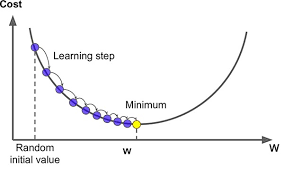
\includegraphics{GD.png}
\caption{alt text}
\end{figure}

\textbf{Error function:}

\$w\_i \to w\_i - \alpha \frac{\partial }{\partial w_i} Error \$

\begin{itemize}
\tightlist
\item
  The plot of the error function is a parabola with weights on x-axis
  and Error on the y-axis.
\item
  Way to descend from large error is to take the derivative or gradient
  of the Error function wrt the weights \(w_i\).
\item
  The gradient points to the direction where the function increases the
  most. Therefore, the negative of this gradient is going to point down
  to the direction where the function decreases the most.
\item
  The error descends in the direction of the negative gradient. This
  means we change the weights \(w_i\) to \$w\_i -
  \alpha \frac{\partial }{\partial w_i} Error \$.
\item
  By multiplying the derivative of the Error term wrt the weights with
  learning rate \((\alpha)\) the step-size is small.
\item
  This means that the error function is decreasing and we're closer to
  the minimum.
\item
  By doing this many times, the result is either a minimum or a pretty
  good value where the error is small which signifies a pretty good
  solution to the linear regression problem.
\end{itemize}

    \hypertarget{mini-gradient-descent}{%
\paragraph{Mini Gradient Descent}\label{mini-gradient-descent}}

\begin{itemize}
\tightlist
\item
  The MAE/MSE minimization is applied to data points all at the same
  time and the process is repeated many times
\end{itemize}

\begin{figure}
\centering
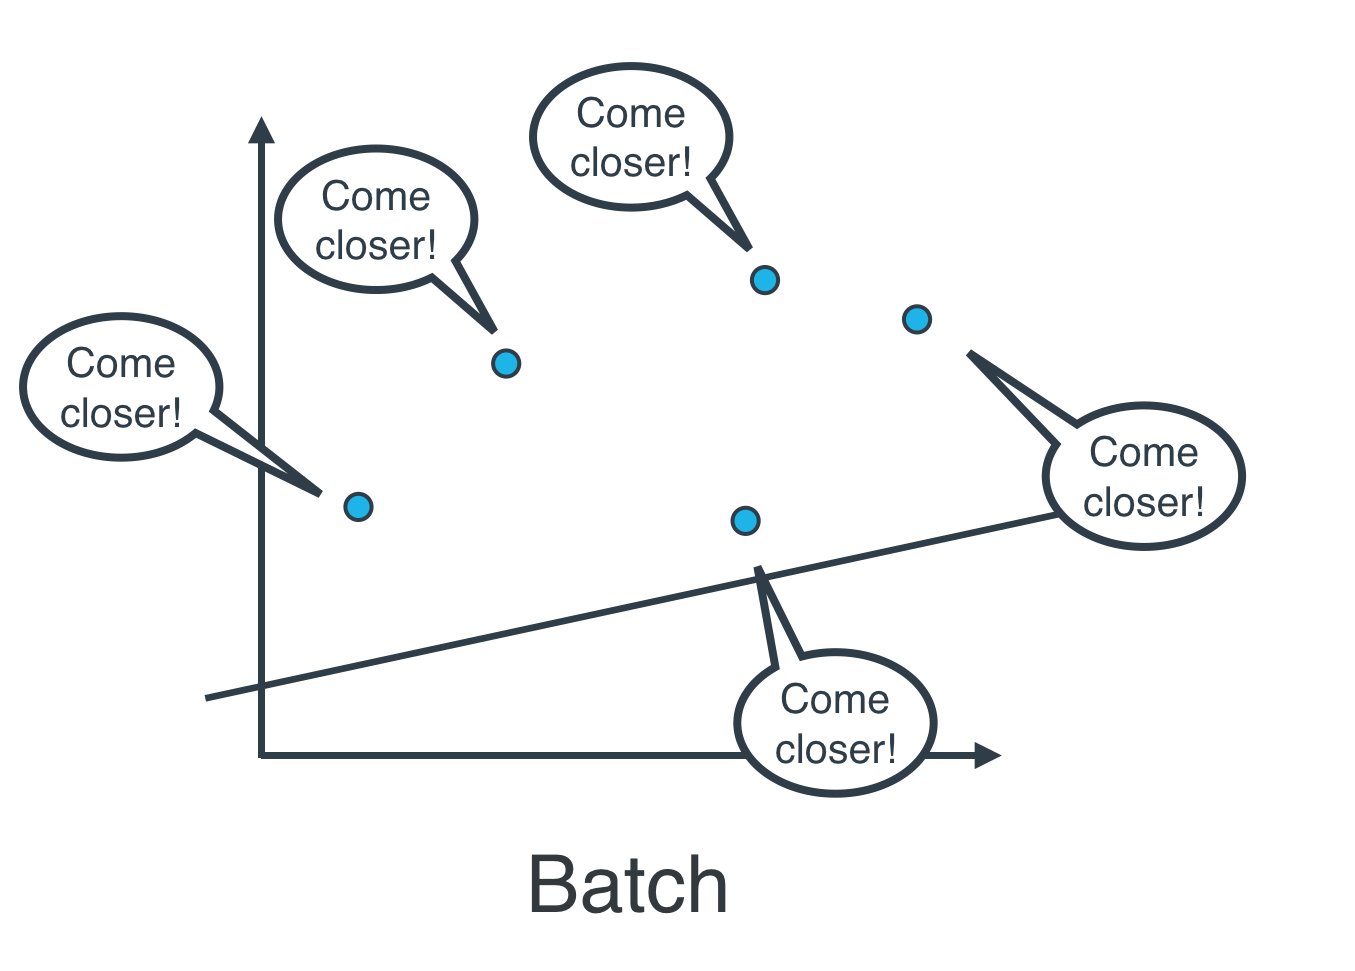
\includegraphics{batch.png}
\caption{alt text}
\end{figure}

    \hypertarget{stochastic-gradient-descent}{%
\paragraph{Stochastic Gradient
Descent}\label{stochastic-gradient-descent}}

\begin{itemize}
\tightlist
\item
  The MAE/MSE minimization is applied to data points one by one and the
  process is repeated many times
\end{itemize}

\begin{figure}
\centering
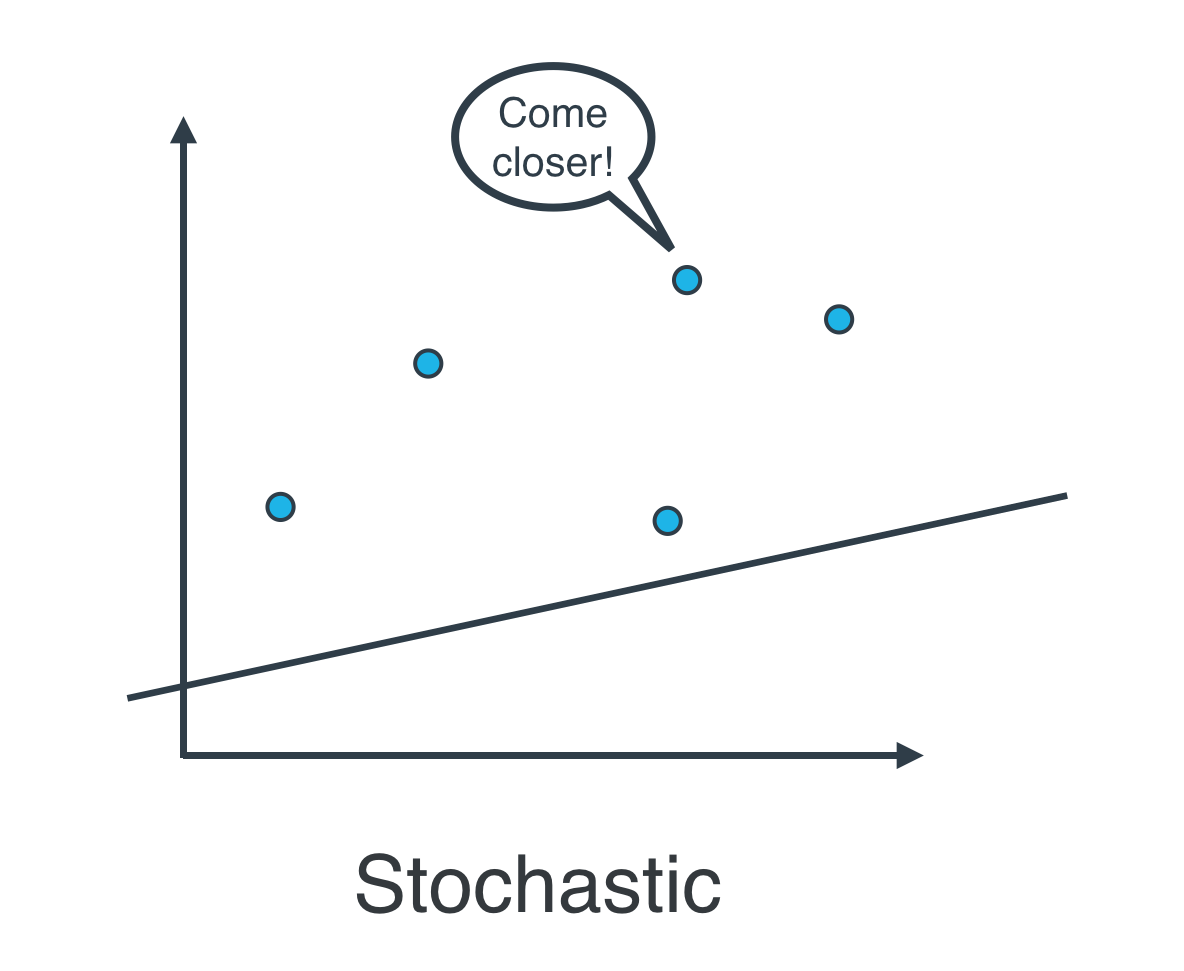
\includegraphics{stochastic.png}
\caption{alt text}
\end{figure}

    \hypertarget{mini-batch-gradient-descent}{%
\paragraph{Mini-Batch Gradient
Descent}\label{mini-batch-gradient-descent}}

\begin{itemize}
\tightlist
\item
  The MAE/MSE minimization is applied to data points into many small
  batches and the process is repeated many times.
\item
  Each batch will have roughly the same number of points and each batch
  is used to update the weights.
\end{itemize}

\begin{figure}
\centering
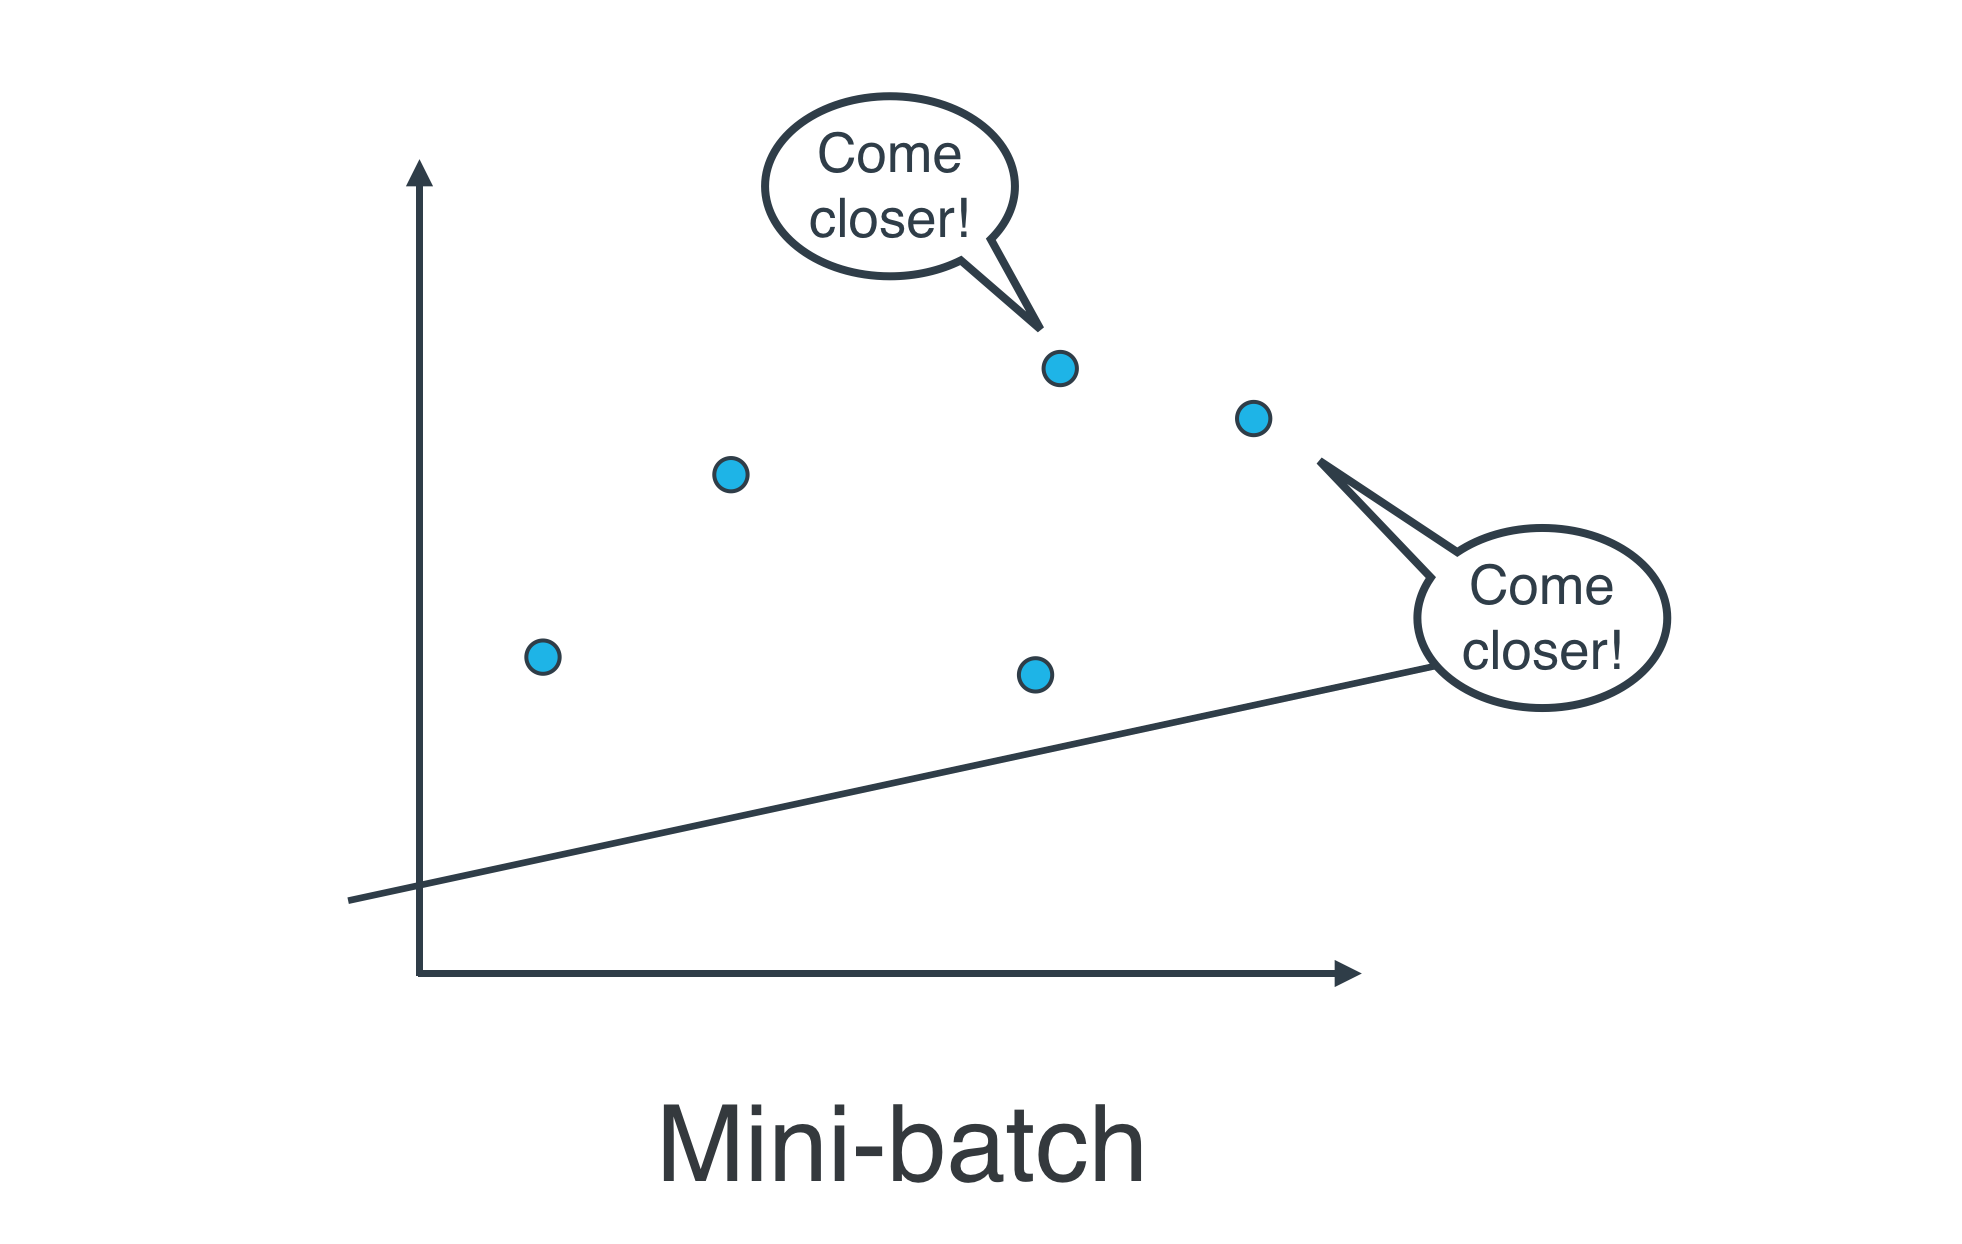
\includegraphics{minibatch.png}
\caption{alt text}
\end{figure}

    \hypertarget{linear-regression-assumptions}{%
\subsubsection{Linear Regression
Assumptions}\label{linear-regression-assumptions}}

\begin{itemize}
\tightlist
\item
  Works best when the data is linear
\item
  Sensitive to outliers
\end{itemize}

    \hypertarget{polynomial-regression}{%
\subsubsection{Polynomial Regression}\label{polynomial-regression}}

Higher order polynomial equations to fit data following a non-linear
trend.

\$ \hat{y} = w\_1x\^{}3 + w\_2x\^{}2 + w\_3x + w\_4 \$

    \hypertarget{complexity-of-model}{%
\subsubsection{Complexity of model}\label{complexity-of-model}}

Simpler models have a tendency to generalize better than complex models.
To make complexity of model into account while measuring the error,
regularization techniques are used.

Total error = Error from misclassification + complexity

\hypertarget{l1-regularization}{%
\paragraph{L1 Regularization}\label{l1-regularization}}

\begin{itemize}
\tightlist
\item
  Takes the coefficients of the model and adds the absolute values to
  the error.
\item
  Computationally inefficient, unless the data is sparse
\item
  Feature selection
\end{itemize}

\hypertarget{l2-regularization}{%
\paragraph{L2 Regularization}\label{l2-regularization}}

\begin{itemize}
\tightlist
\item
  Takes the sum of squares of coefficients of the model and adds the
  value to the error.
\item
  Computationally efficient (computing derivatives of squares is
  efficient), good for non-sparse data
\end{itemize}

    \hypertarget{examples}{%
\subsection{Examples}\label{examples}}

    \begin{Verbatim}[commandchars=\\\{\}]
{\color{incolor}In [{\color{incolor}20}]:} \PY{c+c1}{\PYZsh{} Add import statements}
         \PY{k+kn}{import} \PY{n+nn}{pandas} \PY{k}{as} \PY{n+nn}{pd}
         \PY{k+kn}{from} \PY{n+nn}{sklearn}\PY{n+nn}{.}\PY{n+nn}{linear\PYZus{}model} \PY{k}{import} \PY{n}{LinearRegression}
         
         \PY{c+c1}{\PYZsh{} Assign the dataframe to this variable.}
         \PY{c+c1}{\PYZsh{} TODO: Load the data}
         \PY{n}{bmi\PYZus{}life\PYZus{}data} \PY{o}{=} \PY{n}{pd}\PY{o}{.}\PY{n}{read\PYZus{}csv}\PY{p}{(}\PY{l+s+s1}{\PYZsq{}}\PY{l+s+s1}{bmi\PYZus{}and\PYZus{}life\PYZus{}expectancy.csv}\PY{l+s+s1}{\PYZsq{}}\PY{p}{)}
         \PY{n+nb}{print}\PY{p}{(}\PY{n}{bmi\PYZus{}life\PYZus{}data}\PY{o}{.}\PY{n}{head}\PY{p}{(}\PY{p}{)}\PY{p}{)}
         
         \PY{c+c1}{\PYZsh{} Make and fit the linear regression model}
         \PY{c+c1}{\PYZsh{}TODO: Fit the model and Assign it to bmi\PYZus{}life\PYZus{}model}
         \PY{n}{bmi\PYZus{}life\PYZus{}model} \PY{o}{=} \PY{n}{LinearRegression}\PY{p}{(}\PY{p}{)}
         \PY{n}{bmi\PYZus{}life\PYZus{}model}\PY{o}{.}\PY{n}{fit}\PY{p}{(}\PY{n}{bmi\PYZus{}life\PYZus{}data}\PY{p}{[}\PY{p}{[}\PY{l+s+s1}{\PYZsq{}}\PY{l+s+s1}{BMI}\PY{l+s+s1}{\PYZsq{}}\PY{p}{]}\PY{p}{]}\PY{p}{,} \PY{n}{bmi\PYZus{}life\PYZus{}data}\PY{p}{[}\PY{p}{[}\PY{l+s+s1}{\PYZsq{}}\PY{l+s+s1}{Life expectancy}\PY{l+s+s1}{\PYZsq{}}\PY{p}{]}\PY{p}{]}\PY{p}{)}
         
         \PY{c+c1}{\PYZsh{} Make a prediction using the model}
         \PY{c+c1}{\PYZsh{} TODO: Predict life expectancy for a BMI value of 21.07931}
         \PY{n}{laos\PYZus{}life\PYZus{}exp} \PY{o}{=} \PY{n}{bmi\PYZus{}life\PYZus{}model}\PY{o}{.}\PY{n}{predict}\PY{p}{(}\PY{p}{[}\PY{p}{[}\PY{l+m+mf}{21.07931}\PY{p}{]}\PY{p}{]}\PY{p}{)}
         \PY{n+nb}{print}\PY{p}{(}\PY{l+s+s2}{\PYZdq{}}\PY{l+s+s2}{Life expenctancy: }\PY{l+s+si}{\PYZob{}\PYZcb{}}\PY{l+s+s2}{\PYZdq{}}\PY{o}{.}\PY{n}{format}\PY{p}{(}\PY{n}{laos\PYZus{}life\PYZus{}exp}\PY{p}{)}\PY{p}{)}
\end{Verbatim}


    \begin{Verbatim}[commandchars=\\\{\}]
       Country  Life expectancy       BMI
0  Afghanistan             52.8  20.62058
1      Albania             76.8  26.44657
2      Algeria             75.5  24.59620
3      Andorra             84.6  27.63048
4       Angola             56.7  22.25083
Life expenctancy: [[60.31564716]]

    \end{Verbatim}

    \begin{Verbatim}[commandchars=\\\{\}]
{\color{incolor}In [{\color{incolor}31}]:} \PY{k+kn}{from} \PY{n+nn}{sklearn}\PY{n+nn}{.}\PY{n+nn}{linear\PYZus{}model} \PY{k}{import} \PY{n}{LinearRegression}
         \PY{k+kn}{from} \PY{n+nn}{sklearn}\PY{n+nn}{.}\PY{n+nn}{datasets} \PY{k}{import} \PY{n}{load\PYZus{}boston}
         
         \PY{c+c1}{\PYZsh{} Load the data from the boston house\PYZhy{}prices dataset}
         \PY{n}{boston\PYZus{}data} \PY{o}{=} \PY{n}{load\PYZus{}boston}\PY{p}{(}\PY{p}{)}
         \PY{n}{x} \PY{o}{=} \PY{n}{boston\PYZus{}data}\PY{p}{[}\PY{l+s+s1}{\PYZsq{}}\PY{l+s+s1}{data}\PY{l+s+s1}{\PYZsq{}}\PY{p}{]}
         \PY{n}{y} \PY{o}{=} \PY{n}{boston\PYZus{}data}\PY{p}{[}\PY{l+s+s1}{\PYZsq{}}\PY{l+s+s1}{target}\PY{l+s+s1}{\PYZsq{}}\PY{p}{]}
         \PY{n+nb}{print}\PY{p}{(}\PY{l+s+s1}{\PYZsq{}}\PY{l+s+s1}{X values:}\PY{l+s+se}{\PYZbs{}n}\PY{l+s+s1}{ }\PY{l+s+si}{\PYZob{}\PYZcb{}}\PY{l+s+s1}{\PYZsq{}}\PY{o}{.}\PY{n}{format}\PY{p}{(}\PY{n}{x}\PY{p}{[}\PY{p}{:}\PY{l+m+mi}{1}\PY{p}{]}\PY{p}{)}\PY{p}{)}
         \PY{n+nb}{print}\PY{p}{(}\PY{p}{)}
         \PY{n+nb}{print}\PY{p}{(}\PY{l+s+s1}{\PYZsq{}}\PY{l+s+s1}{Y values:}\PY{l+s+se}{\PYZbs{}n}\PY{l+s+s1}{ }\PY{l+s+si}{\PYZob{}\PYZcb{}}\PY{l+s+s1}{\PYZsq{}}\PY{o}{.}\PY{n}{format}\PY{p}{(}\PY{n}{y}\PY{p}{[}\PY{p}{:}\PY{l+m+mi}{1}\PY{p}{]}\PY{p}{)}\PY{p}{)}
         \PY{n+nb}{print}\PY{p}{(}\PY{p}{)}
         
         \PY{c+c1}{\PYZsh{} Make and fit the linear regression model}
         \PY{n}{lr\PYZus{}model} \PY{o}{=} \PY{n}{LinearRegression}\PY{p}{(}\PY{p}{)}
         \PY{n}{lr\PYZus{}model}\PY{o}{.}\PY{n}{fit}\PY{p}{(}\PY{n}{x}\PY{p}{,}\PY{n}{y}\PY{p}{)}
         
         \PY{c+c1}{\PYZsh{} Make a prediction using the model}
         \PY{n}{sample\PYZus{}house} \PY{o}{=} \PY{p}{[}\PY{p}{[}\PY{l+m+mf}{2.29690000e\PYZhy{}01}\PY{p}{,} \PY{l+m+mf}{0.00000000e+00}\PY{p}{,} \PY{l+m+mf}{1.05900000e+01}\PY{p}{,} \PY{l+m+mf}{0.00000000e+00}\PY{p}{,} \PY{l+m+mf}{4.89000000e\PYZhy{}01}\PY{p}{,}
                         \PY{l+m+mf}{6.32600000e+00}\PY{p}{,} \PY{l+m+mf}{5.25000000e+01}\PY{p}{,} \PY{l+m+mf}{4.35490000e+00}\PY{p}{,} \PY{l+m+mf}{4.00000000e+00}\PY{p}{,} \PY{l+m+mf}{2.77000000e+02}\PY{p}{,}
                         \PY{l+m+mf}{1.86000000e+01}\PY{p}{,} \PY{l+m+mf}{3.94870000e+02}\PY{p}{,} \PY{l+m+mf}{1.09700000e+01}\PY{p}{]}\PY{p}{]}
         
         \PY{c+c1}{\PYZsh{} Predict housing price for the sample\PYZus{}house}
         \PY{n}{prediction} \PY{o}{=} \PY{n}{lr\PYZus{}model}\PY{o}{.}\PY{n}{predict}\PY{p}{(}\PY{n}{sample\PYZus{}house}\PY{p}{)}
         \PY{n+nb}{print}\PY{p}{(}\PY{l+s+s1}{\PYZsq{}}\PY{l+s+s1}{Prediction:}\PY{l+s+se}{\PYZbs{}n}\PY{l+s+s1}{ }\PY{l+s+si}{\PYZob{}\PYZcb{}}\PY{l+s+s1}{\PYZsq{}}\PY{o}{.}\PY{n}{format}\PY{p}{(}\PY{n}{prediction}\PY{p}{)}\PY{p}{)}
\end{Verbatim}


    \begin{Verbatim}[commandchars=\\\{\}]
X values:
 [[6.320e-03 1.800e+01 2.310e+00 0.000e+00 5.380e-01 6.575e+00 6.520e+01
  4.090e+00 1.000e+00 2.960e+02 1.530e+01 3.969e+02 4.980e+00]]

Y values:
 [24.]

Prediction:
 [23.68284712]

    \end{Verbatim}

    \begin{Verbatim}[commandchars=\\\{\}]
{\color{incolor}In [{\color{incolor}2}]:} \PY{k+kn}{from} \PY{n+nn}{sklearn}\PY{n+nn}{.}\PY{n+nn}{model\PYZus{}selection} \PY{k}{import} \PY{n}{KFold}
        \PY{k+kn}{from} \PY{n+nn}{sklearn}\PY{n+nn}{.}\PY{n+nn}{linear\PYZus{}model} \PY{k}{import} \PY{n}{LinearRegression}\PY{p}{,} \PY{n}{Lasso}\PY{p}{,} \PY{n}{Ridge}\PY{p}{,} \PY{n}{ElasticNet}\PY{p}{,} \PY{n}{SGDRegressor}
        \PY{k+kn}{import} \PY{n+nn}{numpy} \PY{k}{as} \PY{n+nn}{np}
        \PY{k+kn}{import} \PY{n+nn}{pylab} \PY{k}{as} \PY{n+nn}{pl}
\end{Verbatim}


    \begin{Verbatim}[commandchars=\\\{\}]
{\color{incolor}In [{\color{incolor}5}]:} \PY{k+kn}{from} \PY{n+nn}{sklearn}\PY{n+nn}{.}\PY{n+nn}{datasets} \PY{k}{import} \PY{n}{load\PYZus{}boston}
        \PY{n}{boston} \PY{o}{=} \PY{n}{load\PYZus{}boston}\PY{p}{(}\PY{p}{)}
        
        \PY{c+c1}{\PYZsh{} In order to do multiple regression we need to add a column of 1s for x0}
        \PY{n}{x} \PY{o}{=} \PY{n}{np}\PY{o}{.}\PY{n}{array}\PY{p}{(}\PY{p}{[}\PY{n}{np}\PY{o}{.}\PY{n}{concatenate}\PY{p}{(}\PY{p}{(}\PY{n}{v}\PY{p}{,}\PY{p}{[}\PY{l+m+mi}{1}\PY{p}{]}\PY{p}{)}\PY{p}{)} \PY{k}{for} \PY{n}{v} \PY{o+ow}{in} \PY{n}{boston}\PY{o}{.}\PY{n}{data}\PY{p}{]}\PY{p}{)}
        \PY{n}{y} \PY{o}{=} \PY{n}{boston}\PY{o}{.}\PY{n}{target}
        
        \PY{n}{np}\PY{o}{.}\PY{n}{set\PYZus{}printoptions}\PY{p}{(}\PY{n}{precision}\PY{o}{=}\PY{l+m+mi}{2}\PY{p}{,} \PY{n}{linewidth}\PY{o}{=}\PY{l+m+mi}{120}\PY{p}{,} \PY{n}{suppress}\PY{o}{=}\PY{k+kc}{True}\PY{p}{,} \PY{n}{edgeitems}\PY{o}{=}\PY{l+m+mi}{4}\PY{p}{)}
\end{Verbatim}


    \begin{Verbatim}[commandchars=\\\{\}]
{\color{incolor}In [{\color{incolor}6}]:} \PY{c+c1}{\PYZsh{} Create linear regression object}
        \PY{n}{linreg} \PY{o}{=} \PY{n}{LinearRegression}\PY{p}{(}\PY{p}{)}
        
        \PY{c+c1}{\PYZsh{} Train the model using the training sets}
        \PY{n}{linreg}\PY{o}{.}\PY{n}{fit}\PY{p}{(}\PY{n}{x}\PY{p}{,}\PY{n}{y}\PY{p}{)}
\end{Verbatim}


\begin{Verbatim}[commandchars=\\\{\}]
{\color{outcolor}Out[{\color{outcolor}6}]:} LinearRegression(copy\_X=True, fit\_intercept=True, n\_jobs=None,
                 normalize=False)
\end{Verbatim}
            
    \begin{Verbatim}[commandchars=\\\{\}]
{\color{incolor}In [{\color{incolor}7}]:} \PY{c+c1}{\PYZsh{} Let\PYZsq{}s see predictions for the first 10 instances}
        \PY{n+nb}{print}\PY{p}{(}\PY{n}{linreg}\PY{o}{.}\PY{n}{predict}\PY{p}{(}\PY{n}{x}\PY{p}{[}\PY{p}{:}\PY{l+m+mi}{10}\PY{p}{]}\PY{p}{)}\PY{p}{)}
\end{Verbatim}


    \begin{Verbatim}[commandchars=\\\{\}]
[30.   25.03 30.57 28.61 27.94 25.26 23.   19.54 11.52 18.92]

    \end{Verbatim}

    \begin{Verbatim}[commandchars=\\\{\}]
{\color{incolor}In [{\color{incolor}9}]:} \PY{c+c1}{\PYZsh{} Compute RMSE on training data}
        \PY{c+c1}{\PYZsh{} p = np.array([linreg.predict(xi) for xi in x])}
        \PY{n}{p} \PY{o}{=} \PY{n}{linreg}\PY{o}{.}\PY{n}{predict}\PY{p}{(}\PY{n}{x}\PY{p}{)}
        \PY{c+c1}{\PYZsh{} Now we can constuct a vector of errors}
        \PY{n}{err} \PY{o}{=} \PY{n+nb}{abs}\PY{p}{(}\PY{n}{p}\PY{o}{\PYZhy{}}\PY{n}{y}\PY{p}{)}
        
        \PY{c+c1}{\PYZsh{} Let\PYZsq{}s see the error on the first 10 predictions}
        \PY{n+nb}{print}\PY{p}{(}\PY{n}{err}\PY{p}{[}\PY{p}{:}\PY{l+m+mi}{10}\PY{p}{]}\PY{p}{)}
\end{Verbatim}


    \begin{Verbatim}[commandchars=\\\{\}]
[6.   3.43 4.13 4.79 8.26 3.44 0.1  7.56 4.98 0.02]

    \end{Verbatim}

    \begin{Verbatim}[commandchars=\\\{\}]
{\color{incolor}In [{\color{incolor}10}]:} \PY{c+c1}{\PYZsh{} Dot product of error vector with itself gives us the sum of squared errors}
         \PY{n}{total\PYZus{}error} \PY{o}{=} \PY{n}{np}\PY{o}{.}\PY{n}{dot}\PY{p}{(}\PY{n}{err}\PY{p}{,}\PY{n}{err}\PY{p}{)}
         \PY{c+c1}{\PYZsh{} Compute RMSE}
         \PY{n}{rmse\PYZus{}train} \PY{o}{=} \PY{n}{np}\PY{o}{.}\PY{n}{sqrt}\PY{p}{(}\PY{n}{total\PYZus{}error}\PY{o}{/}\PY{n+nb}{len}\PY{p}{(}\PY{n}{p}\PY{p}{)}\PY{p}{)}
         \PY{n+nb}{print}\PY{p}{(}\PY{n}{rmse\PYZus{}train}\PY{p}{)}
\end{Verbatim}


    \begin{Verbatim}[commandchars=\\\{\}]
4.679191295697281

    \end{Verbatim}

    \begin{Verbatim}[commandchars=\\\{\}]
{\color{incolor}In [{\color{incolor}12}]:} \PY{c+c1}{\PYZsh{} We can view the regression coefficients}
         \PY{n+nb}{print}\PY{p}{(}\PY{l+s+s1}{\PYZsq{}}\PY{l+s+s1}{Regression Coefficients: }\PY{l+s+se}{\PYZbs{}n}\PY{l+s+s1}{\PYZsq{}}\PY{p}{,} \PY{n}{linreg}\PY{o}{.}\PY{n}{coef\PYZus{}}\PY{p}{)}
\end{Verbatim}


    \begin{Verbatim}[commandchars=\\\{\}]
Regression Coefficients: 
 [ -0.11   0.05   0.02   2.69 -17.77   3.81   0.    -1.48   0.31  -0.01  -0.95   0.01  -0.52   0.  ]

    \end{Verbatim}

    \begin{Verbatim}[commandchars=\\\{\}]
{\color{incolor}In [{\color{incolor}13}]:} \PY{c+c1}{\PYZsh{} Plot outputs}
         \PY{o}{\PYZpc{}}\PY{k}{matplotlib} inline
         \PY{n}{pl}\PY{o}{.}\PY{n}{plot}\PY{p}{(}\PY{n}{p}\PY{p}{,} \PY{n}{y}\PY{p}{,}\PY{l+s+s1}{\PYZsq{}}\PY{l+s+s1}{ro}\PY{l+s+s1}{\PYZsq{}}\PY{p}{)}
         \PY{n}{pl}\PY{o}{.}\PY{n}{plot}\PY{p}{(}\PY{p}{[}\PY{l+m+mi}{0}\PY{p}{,}\PY{l+m+mi}{50}\PY{p}{]}\PY{p}{,}\PY{p}{[}\PY{l+m+mi}{0}\PY{p}{,}\PY{l+m+mi}{50}\PY{p}{]}\PY{p}{,} \PY{l+s+s1}{\PYZsq{}}\PY{l+s+s1}{g\PYZhy{}}\PY{l+s+s1}{\PYZsq{}}\PY{p}{)}
         \PY{n}{pl}\PY{o}{.}\PY{n}{xlabel}\PY{p}{(}\PY{l+s+s1}{\PYZsq{}}\PY{l+s+s1}{predicted}\PY{l+s+s1}{\PYZsq{}}\PY{p}{)}
         \PY{n}{pl}\PY{o}{.}\PY{n}{ylabel}\PY{p}{(}\PY{l+s+s1}{\PYZsq{}}\PY{l+s+s1}{real}\PY{l+s+s1}{\PYZsq{}}\PY{p}{)}
         \PY{n}{pl}\PY{o}{.}\PY{n}{show}\PY{p}{(}\PY{p}{)}
\end{Verbatim}


    \begin{center}
    \adjustimage{max size={0.9\linewidth}{0.9\paperheight}}{output_28_0.png}
    \end{center}
    { \hspace*{\fill} \\}
    
    \hypertarget{ridge-regression}{%
\paragraph{Ridge Regression}\label{ridge-regression}}

    \begin{Verbatim}[commandchars=\\\{\}]
{\color{incolor}In [{\color{incolor}14}]:} \PY{c+c1}{\PYZsh{} Create linear regression object with a ridge coefficient 0.5}
         \PY{n}{ridge} \PY{o}{=} \PY{n}{Ridge}\PY{p}{(}\PY{n}{fit\PYZus{}intercept}\PY{o}{=}\PY{k+kc}{True}\PY{p}{,} \PY{n}{alpha}\PY{o}{=}\PY{l+m+mf}{0.5}\PY{p}{)}
         
         \PY{c+c1}{\PYZsh{} Train the model using the training set}
         \PY{n}{ridge}\PY{o}{.}\PY{n}{fit}\PY{p}{(}\PY{n}{x}\PY{p}{,}\PY{n}{y}\PY{p}{)}
\end{Verbatim}


\begin{Verbatim}[commandchars=\\\{\}]
{\color{outcolor}Out[{\color{outcolor}14}]:} Ridge(alpha=0.5, copy\_X=True, fit\_intercept=True, max\_iter=None,
            normalize=False, random\_state=None, solver='auto', tol=0.001)
\end{Verbatim}
            
    \begin{Verbatim}[commandchars=\\\{\}]
{\color{incolor}In [{\color{incolor}16}]:} \PY{c+c1}{\PYZsh{} Compute RMSE on training data}
         \PY{c+c1}{\PYZsh{} p = np.array([ridge.predict(xi) for xi in x])}
         \PY{n}{p} \PY{o}{=} \PY{n}{ridge}\PY{o}{.}\PY{n}{predict}\PY{p}{(}\PY{n}{x}\PY{p}{)}
         \PY{n}{err} \PY{o}{=} \PY{n}{p}\PY{o}{\PYZhy{}}\PY{n}{y}
         \PY{n}{total\PYZus{}error} \PY{o}{=} \PY{n}{np}\PY{o}{.}\PY{n}{dot}\PY{p}{(}\PY{n}{err}\PY{p}{,}\PY{n}{err}\PY{p}{)}
         \PY{n}{rmse\PYZus{}train} \PY{o}{=} \PY{n}{np}\PY{o}{.}\PY{n}{sqrt}\PY{p}{(}\PY{n}{total\PYZus{}error}\PY{o}{/}\PY{n+nb}{len}\PY{p}{(}\PY{n}{p}\PY{p}{)}\PY{p}{)}
         
         \PY{n}{method\PYZus{}name} \PY{o}{=} \PY{l+s+s1}{\PYZsq{}}\PY{l+s+s1}{Ridge Regression}\PY{l+s+s1}{\PYZsq{}}
         \PY{n+nb}{print}\PY{p}{(}\PY{l+s+s1}{\PYZsq{}}\PY{l+s+s1}{Method: }\PY{l+s+si}{\PYZpc{}s}\PY{l+s+s1}{\PYZsq{}} \PY{o}{\PYZpc{}}\PY{k}{method\PYZus{}name})
         \PY{n+nb}{print}\PY{p}{(}\PY{l+s+s1}{\PYZsq{}}\PY{l+s+s1}{RMSE on training: }\PY{l+s+si}{\PYZpc{}.4f}\PY{l+s+s1}{\PYZsq{}} \PY{o}{\PYZpc{}}\PY{k}{rmse\PYZus{}train})
\end{Verbatim}


    \begin{Verbatim}[commandchars=\\\{\}]
Method: Ridge Regression
RMSE on training: 4.6854

    \end{Verbatim}

    \hypertarget{regression-using-stochastic-gradeint-descent}{%
\paragraph{Regression using Stochastic Gradeint
Descent}\label{regression-using-stochastic-gradeint-descent}}

    \begin{Verbatim}[commandchars=\\\{\}]
{\color{incolor}In [{\color{incolor}19}]:} \PY{c+c1}{\PYZsh{} SGD is very senstitive to varying\PYZhy{}sized feature values. So, first we need to do feature scaling.}
         
         \PY{k+kn}{from} \PY{n+nn}{sklearn}\PY{n+nn}{.}\PY{n+nn}{preprocessing} \PY{k}{import} \PY{n}{StandardScaler}
         
         \PY{n}{scaler} \PY{o}{=} \PY{n}{StandardScaler}\PY{p}{(}\PY{p}{)}
         \PY{n}{scaler}\PY{o}{.}\PY{n}{fit}\PY{p}{(}\PY{n}{x}\PY{p}{)}
         \PY{n}{x\PYZus{}s} \PY{o}{=} \PY{n}{scaler}\PY{o}{.}\PY{n}{transform}\PY{p}{(}\PY{n}{x}\PY{p}{)}
         
         \PY{n}{sgdreg} \PY{o}{=} \PY{n}{SGDRegressor}\PY{p}{(}\PY{n}{penalty}\PY{o}{=}\PY{l+s+s1}{\PYZsq{}}\PY{l+s+s1}{l2}\PY{l+s+s1}{\PYZsq{}}\PY{p}{,} \PY{n}{alpha}\PY{o}{=}\PY{l+m+mf}{0.15}\PY{p}{,} \PY{n}{max\PYZus{}iter}\PY{o}{=}\PY{l+m+mi}{200}\PY{p}{)}
         
         \PY{c+c1}{\PYZsh{} Compute RMSE on training data}
         \PY{n}{sgdreg}\PY{o}{.}\PY{n}{fit}\PY{p}{(}\PY{n}{x\PYZus{}s}\PY{p}{,}\PY{n}{y}\PY{p}{)}
         \PY{n}{p} \PY{o}{=} \PY{n}{sgdreg}\PY{o}{.}\PY{n}{predict}\PY{p}{(}\PY{n}{x\PYZus{}s}\PY{p}{)}
         \PY{n}{err} \PY{o}{=} \PY{n}{p}\PY{o}{\PYZhy{}}\PY{n}{y}
         \PY{n}{total\PYZus{}error} \PY{o}{=} \PY{n}{np}\PY{o}{.}\PY{n}{dot}\PY{p}{(}\PY{n}{err}\PY{p}{,}\PY{n}{err}\PY{p}{)}
         \PY{n}{rmse\PYZus{}train} \PY{o}{=} \PY{n}{np}\PY{o}{.}\PY{n}{sqrt}\PY{p}{(}\PY{n}{total\PYZus{}error}\PY{o}{/}\PY{n+nb}{len}\PY{p}{(}\PY{n}{p}\PY{p}{)}\PY{p}{)}
         
         \PY{n}{method\PYZus{}name} \PY{o}{=} \PY{l+s+s1}{\PYZsq{}}\PY{l+s+s1}{Stochastic Gradient Descent Regression}\PY{l+s+s1}{\PYZsq{}}
         \PY{n+nb}{print}\PY{p}{(}\PY{l+s+s1}{\PYZsq{}}\PY{l+s+s1}{Method: }\PY{l+s+si}{\PYZpc{}s}\PY{l+s+s1}{\PYZsq{}} \PY{o}{\PYZpc{}}\PY{k}{method\PYZus{}name})
         \PY{n+nb}{print}\PY{p}{(}\PY{l+s+s1}{\PYZsq{}}\PY{l+s+s1}{RMSE on training: }\PY{l+s+si}{\PYZpc{}.4f}\PY{l+s+s1}{\PYZsq{}} \PY{o}{\PYZpc{}}\PY{k}{rmse\PYZus{}train})
\end{Verbatim}


    \begin{Verbatim}[commandchars=\\\{\}]
Method: Stochastic Gradient Descent Regression
RMSE on training: 4.8071

    \end{Verbatim}

    \begin{Verbatim}[commandchars=\\\{\}]
C:\textbackslash{}Users\textbackslash{}lsurampudi\textbackslash{}Anaconda3\textbackslash{}envs\textbackslash{}py36\textbackslash{}lib\textbackslash{}site-packages\textbackslash{}sklearn\textbackslash{}linear\_model\textbackslash{}stochastic\_gradient.py:183: FutureWarning: max\_iter and tol parameters have been added in SGDRegressor in 0.19. If max\_iter is set but tol is left unset, the default value for tol in 0.19 and 0.20 will be None (which is equivalent to -infinity, so it has no effect) but will change in 0.21 to 1e-3. Specify tol to silence this warning.
  FutureWarning)

    \end{Verbatim}


    % Add a bibliography block to the postdoc
    
    
    
    \end{document}
